\documentclass[10pt,a4paper]{article}
\usepackage[margin=2cm]{geometry}
\usepackage{graphicx}
\usepackage{booktabs}
\usepackage{amsmath}
\usepackage[hidelinks]{hyperref}
\usepackage{caption}
\captionsetup{font=small,labelfont=bf}
\setlength{\parskip}{0.3em}
\setlength{\parindent}{0pt}
\graphicspath{{figures/}}
\pagestyle{empty}

\title{\vspace{-2.2em}\textbf{Green Window Observatory:\\[-0.1em]
Carbon-Intensity Forecasting for Carbon-Aware Workload Scheduling}}
\author{\normalsize Green Decision Module. Technical Note, V1.0}
\date{\vspace{-1em}\small\today}

\begin{document}
\maketitle
\vspace{-2em}

\begin{abstract}\small\noindent
A reproducible, open-data model forecasts the carbon intensity of the French
grid and ranks upcoming low-carbon time windows, to support carbon-aware
scheduling of deferrable workloads. A direct multi-horizon gradient-boosting
model, trained on open RTE/ODRE data and free weather forecasts (Open-Meteo),
captures 67\% (48\,h) and 73\% (24\,h) of the savings achievable between naive
execution and perfect foresight, under a leakage-free rolling-origin backtest.
The model is fully open and vendor-free.
\end{abstract}

\section{Purpose}
The system addresses a bounded scheduling question: \emph{over the next
1--48\,h, which candidate times have the lowest carbon intensity?} It produces
an hourly carbon-intensity forecast for the French bidding zone and a ranked set
of low-carbon \emph{windows}. A scheduler or Kubernetes integration can then
defer batch workloads, such as Monte-Carlo runs or offline training and
inference, to lower-carbon hours. Per-workload actions (suspend, power-cap,
co-locate) are out of scope for this version.

\section{Data}
The ground truth is RTE \texttt{taux\_co2}, a production-based carbon intensity
(gCO$_2$/kWh) from the open ODRE/eCO2mix portal, aggregated to hourly UTC over
$\sim$5 years; the generation mix is available as features. Ranking green hours
requires knowing \emph{what will happen}; in France this is driven mainly by
wind, so the model uses \emph{forecast} features at the target time~$T$, all
obtainable in real time and leakage-free:

\begin{center}\small
\begin{tabular}{@{}lll@{}}
\toprule
Feature & Source & Real-time availability \\
\midrule
Wind speed @100\,m & Open-Meteo (free, no key) & forecast to 16 days, all horizons \\
Solar irradiance & Open-Meteo & same \\
Consumption forecast & RTE \texttt{prevision\_j1} & day-ahead, gated to $\le 24$\,h \\
\bottomrule
\end{tabular}
\end{center}

A forecast for $T$ is published before $T$, so using it at decision time
$t_0<T$ is not leakage; the realized value $y(t_0{+}h)$ is used only as a label.

\section{Forecasting model}
A \textbf{direct multi-horizon} regressor: six independent gradient-boosted tree
estimators (\texttt{HistGradientBoosting}), one per horizon
$h\in\{1,3,6,12,24,48\}$\,h. Each estimator uses about 37 features that are known
at $t_0$ or deterministic: the target-time calendar, the recent signal (lags,
rolling means, slope, residual from climatology), the system state at $t_0$, and
the target-time forecast features above. For a given horizon, examples
$(X=\text{features at }t_0,\; y=\text{intensity at }t_0{+}h)$ are fit on data
before the test period. At prediction time each estimator emits its horizon in a
single pass from one origin, so overlapping horizons stay consistent. Recursive
forecasting is avoided, since it would also require forecasting the mix. Gradient
boosting is preferred over ARIMA or deep learning because the problem is tabular
with nonlinear calendar$\times$weather interactions, it handles missing values
natively, and it stays fast and explainable.

\section{Low-carbon windows}
Each forecast is mapped to a green score in $[0,1]$ (higher is greener) by
inverting the empirical CDF within the horizon, $\text{green\_score}(x)=1-F_H(x)$,
which is robust to the skew of carbon data. A low-carbon window is a contiguous
block below a percentile of the horizon, gap-merged and duration-filtered, ranked
by mean green score.

\section{Evaluation and metrics}
\textbf{Protocol.} A leakage-free \emph{rolling-origin} backtest: fit on data
before 2026-02-01 ($44{,}563$ hourly rows); advance an origin every 6\,h over
Feb--Apr 2026 (348 origins), predicting all horizons from information up to the
origin only.

\textbf{Point accuracy.} MAE, RMSE, bias, and a relative error using WAPE rather
than MAPE, $\text{WAPE}=\sum_i|\hat y_i-y_i|/\sum_i|y_i|$. MAPE weights each hour
by the inverse of its own magnitude, so on a grid that is usually at low
intensity (5--15\,gCO$_2$/kWh) it is dominated by already-clean hours and diverges
as $y\!\to\!0$; WAPE normalizes total error by total intensity and is stable.

\textbf{Decision quality (operational metric).} Each strategy selects the hour it
predicts greenest within the horizon; the realized intensity there is compared to
run-now ($C_{\text{now}}$) and perfect foresight ($C_{\text{PF}}$), which selects
on realized values and is an upper bound. The reported metrics are mean realized intensity, regret
$C_{\text{model}}-C_{\text{PF}}$, Spearman rank correlation, top-1 accuracy, and
the share of achievable savings captured,
$\;(C_{\text{now}}-C_{\text{model}})/(C_{\text{now}}-C_{\text{PF}})\times 100$,
which is 0\% for run-now and 100\% for perfect foresight.

\section{Results}
The ML model dominates the baseline ladder on decision quality
(Table~\ref{tab:decision}), capturing 67\% of perfect-foresight potential at
48\,h and 73\% at the primary 24\,h horizon. The wind/solar forecast features are
the main driver, raising Spearman from 0.23 to 0.34 and cutting 48\,h relative
error from 37.7\% to 30.3\% WAPE (Table~\ref{tab:wape}; global WAPE 18\%).
Following the selected ML window yields $\sim$13\% lower carbon intensity than
immediate execution in the reference test period.

\begin{table}[h]\centering\small
\caption{Green-window selection over 348 origins (Feb--Apr 2026). Realized/regret
in gCO$_2$/kWh; PF = perfect foresight.}
\label{tab:decision}
\begin{tabular}{@{}lrrrrr@{}}
\toprule
Strategy & Realized & Regret & \% of PF & Spearman & Top-1 \\
\midrule
Run-now              & 14.91 & 3.16 & 0.0   & --   & --   \\
Persistence          & 15.04 & 3.29 & $-4.1$& --   & 0.24 \\
Climatology          & 13.85 & 2.09 & 33.7  & 0.05 & 0.20 \\
Corrected clim.      & 13.36 & 1.61 & 49.1  & 0.05 & 0.26 \\
SARIMAX              & 13.36 & 1.60 & 49.2  & 0.16 & 0.25 \\
\textbf{ML model} & \textbf{12.80} & \textbf{1.04} & \textbf{67.0} & \textbf{0.34} & \textbf{0.41} \\
Perfect foresight    & 11.76 & 0.00 & 100.0 & 1.00 & 1.00 \\
\bottomrule
\end{tabular}
\end{table}

\begin{table}[h]\centering\small
\caption{Relative point error (WAPE, \%) by forecast horizon.}
\label{tab:wape}
\begin{tabular}{@{}lrrrrrr@{}}
\toprule
Model & 1\,h & 3\,h & 6\,h & 12\,h & 24\,h & 48\,h \\
\midrule
Persistence      & 5.3 & 12.1 & 26.9 & 22.3 & 21.9 & 26.1 \\
Corrected clim.  & 34.1 & 35.2 & 40.6 & 49.6 & 68.6 & 94.8 \\
\textbf{ML model} & \textbf{5.5} & \textbf{10.7} & \textbf{18.5} & \textbf{20.3} & \textbf{24.0} & \textbf{30.3} \\
\bottomrule
\end{tabular}
\end{table}

\begin{figure}[h]\centering
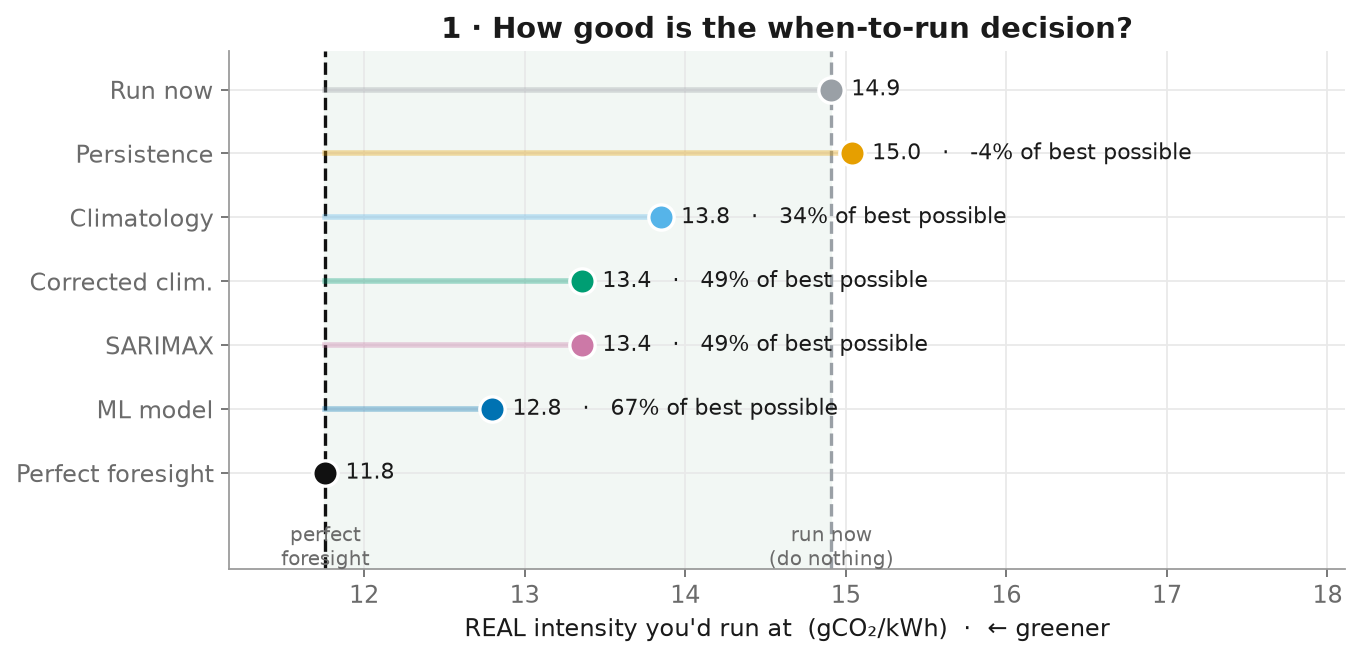
\includegraphics[width=0.58\linewidth]{1_decision_quality.png}
\caption{Realized carbon intensity per strategy, bounded by run-now and perfect
foresight; the ML model captures 67\% of the gap.}
\label{fig:decision}
\end{figure}

\begin{figure}[h]\centering
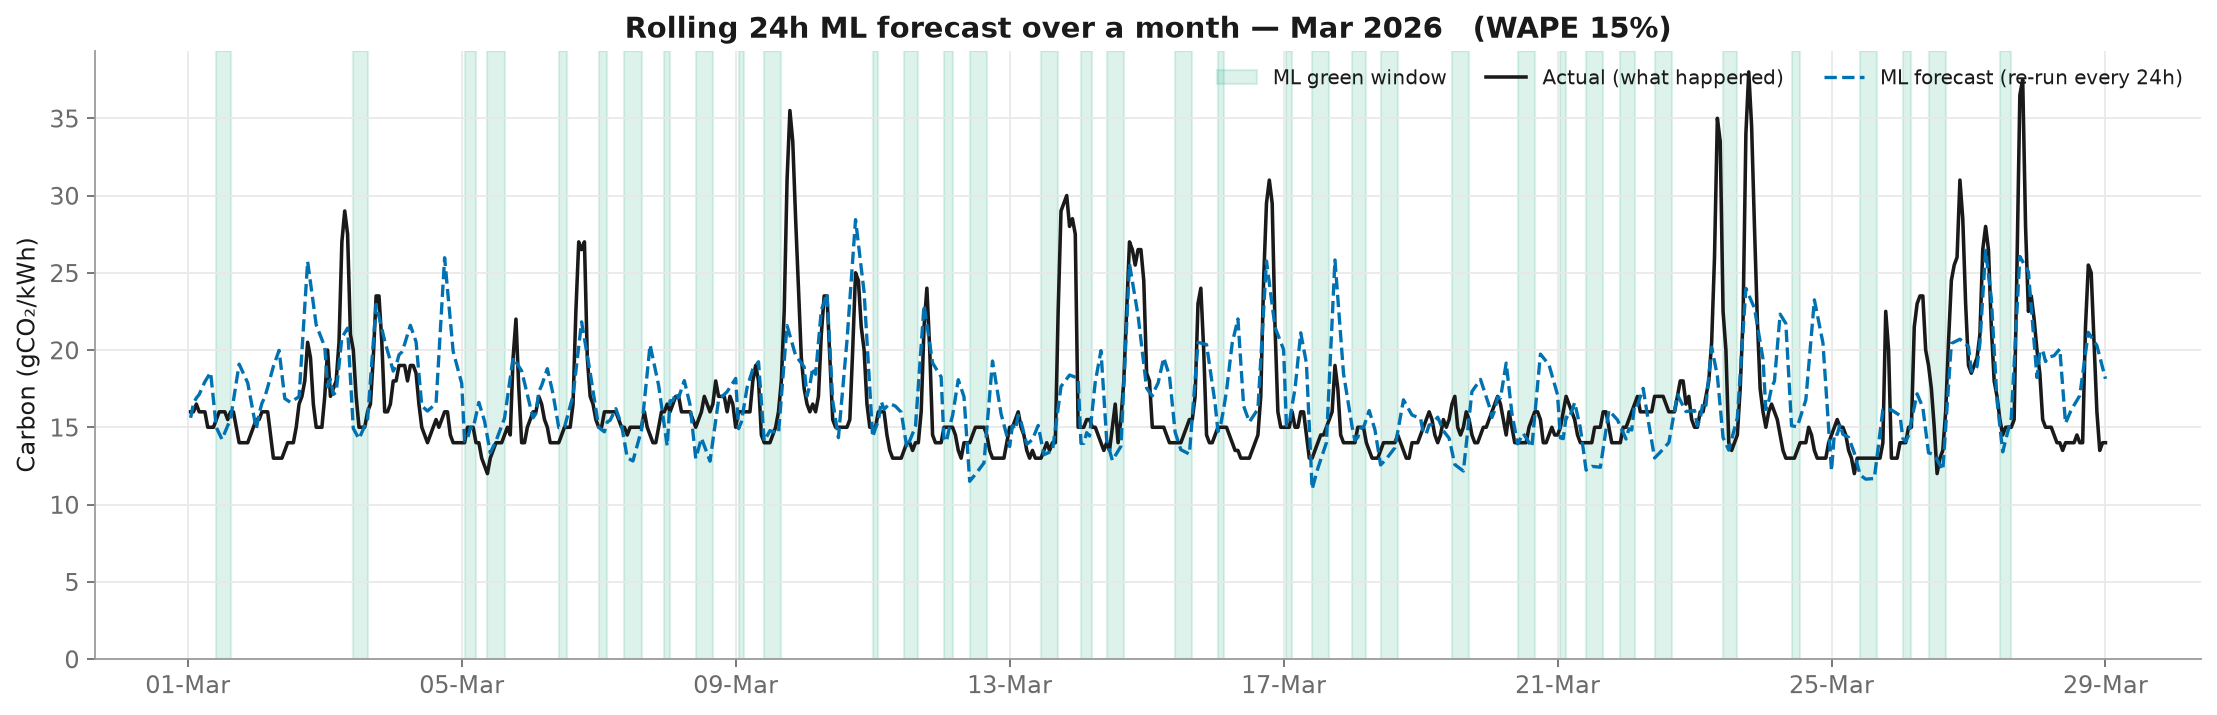
\includegraphics[width=0.74\linewidth]{month_2026-03.png}
\caption{Operational view: a 24\,h ML forecast re-issued every day across a
representative month (March 2026, WAPE 15\%). Black = realized, dashed = forecast,
shading = predicted low-carbon windows.}
\label{fig:month}
\end{figure}

\section{Comparison with external providers}
A direct backtest against a commercial provider (e.g.\ Electricity Maps) is not
feasible: their historical forecasts are not exposed for replay, and they report
a consumption-based intensity (a different accounting basis), so absolute values
are not comparable; a live comparison shows $\sim$0.7 Spearman agreement between
the two 24\,h forecasts. The module is built entirely from free, open data with
no vendor dependency, and each prediction is reproducible and auditable.

\section{Conclusion}
The model is a reproducible, open carbon-forecasting layer that ranks upcoming
low-carbon windows and captures most of the savings that perfect foresight
could achieve. The current ceiling is ranking quality (Spearman $0.34$). Future
improvements should focus on richer weather features and ranking-aware training
objectives as prerequisites for workload-level scheduling decisions.

\end{document}
